\documentclass[11pt,a4paper]{article}

\usepackage[T1]{fontenc}
% Zotero exports some CHI/IUI series fields with a Unicode prime (IUI′15).
\DeclareUnicodeCharacter{2032}{'}
\usepackage[default]{sourceserifpro}
\usepackage{sourcesanspro}
\usepackage[margin=2.2cm]{geometry}
\usepackage{microtype}
\usepackage[table]{xcolor}
\usepackage{caption}
\usepackage{titlesec}
\usepackage{cite}
\usepackage{tikz}
\usetikzlibrary{positioning,arrows.meta,fit,calc}

\definecolor{inkprimary}{HTML}{1A1A19}
\definecolor{inkmuted}{HTML}{52514E}
\definecolor{gridline}{HTML}{E6E5E2}
\definecolor{accent}{HTML}{2A78D6}
\color{inkprimary}

\captionsetup{font=footnotesize}
\titleformat{\section}{\normalfont\sffamily\large\bfseries}{}{0em}{}
\titlespacing*{\section}{0pt}{1.1ex}{0.5ex}
\setlength{\parskip}{0.45ex}

\usepackage[hidelinks]{hyperref}
\hypersetup{
  pdftitle  = {Your Camera Roll, Your Story: Selection and Storytelling with Adjustable AI Help},
  pdfauthor = {Kashyap Shankar Iyer},
}

% Counted words: body text from \section{Problem and context} to the end of
% \section{Possible contribution}. Figure, caption, title and references are
% excluded by the brief and wrapped in %TC:ignore. Recount with:
%   texcount -inc -sum Kashyap_3087617_Literature_Review.tex
\newcommand{\wordcount}{737}

\begin{document}

%TC:ignore
\begin{center}
  {\sffamily\Large\bfseries Your Camera Roll, Your Story:\\
  Selection and Storytelling with Adjustable AI Help}\\[1ex]
  {\sffamily Kashyap Shankar Iyer (3087617) \quad·\quad Intelligent Interactive Systems,
  Assignment~1: Literature Review}\\[0.4ex]
  {\sffamily\bfseries Word count: \wordcount}
\end{center}
%TC:endignore

\section{Problem and context}

After a trip, people hold hundreds of photos they want to share. A social media post asks for
two things: choosing a few photos and writing words that fit them.

Generative AI can now help with both, and how much it writes can vary. Draxler
et al.\ compared four ways of producing a postcard from a trip: writing it
themselves, editing AI text, choosing between AI texts, or getting a text the AI wrote
in full~\cite{draxler_ai_2024}. A personal post is how people present themselves, so it matters where on this
range a post sits. This review asks how AI can help a person turn a trip album
into posts when the person chooses how much of the writing the AI does. It
is relevant to anyone sharing personal memories through AI tools.

\section{Related work}

\textbf{Telling stories with photos} (Figure~\ref{fig:map}). Balabanović et al.\
found that people tell photo stories in two ways: \emph{photo-driven}, where each
photo prompts the story, and \emph{story-driven}, where the story leads and
photos are found to fit it~\cite{balabanovic_storytelling_2000}. Their
participants told stories aloud with a prototype device, so the study shows that
story-driven telling happens, not how AI could support it.

\textbf{AI writes from photos.} VIST, a visual storytelling dataset, pairs
20,211 photo sequences with crowd-written stories so models can learn to generate
them~\cite{huang_visual_2016}. Because crowd
workers wrote these stories about other people's photos, the target is a typical
story, not the voice of the person who took them.

\textbf{Co-writing and ownership.} In Draxler et al.'s study, ownership was low
for AI-generated text and rose with the person's influence over it, yet people
rarely declared AI authorship~\cite{draxler_ai_2024}. An opinionated assistant
shifted both what participants wrote in a social media post and their later
views~\cite{jakesch_co-writing_2023}. Vistoria, which combines text and image
editing for fiction, measurably raised writers' workload, and most of its 12
participants said in interviews that they felt more ownership than with a
text-only baseline~\cite{fu_vistoria_2026-1}. Together these studies show
that AI help changes both how far people feel a text is theirs and what it
says.

\textbf{Design principles.} Mixed-initiative systems should account for
uncertainty and make correction cheap~\cite{horvitz_principles_1999}. In Kulesza
et al.'s study, explanations users could act on helped them correct a classifier
up to twice as efficiently~\cite{kulesza_principles_2015}. Together they suggest
that each match should come with a checkable reason and a way to swap it.

%TC:ignore
\begin{figure}[!hb]
\centering
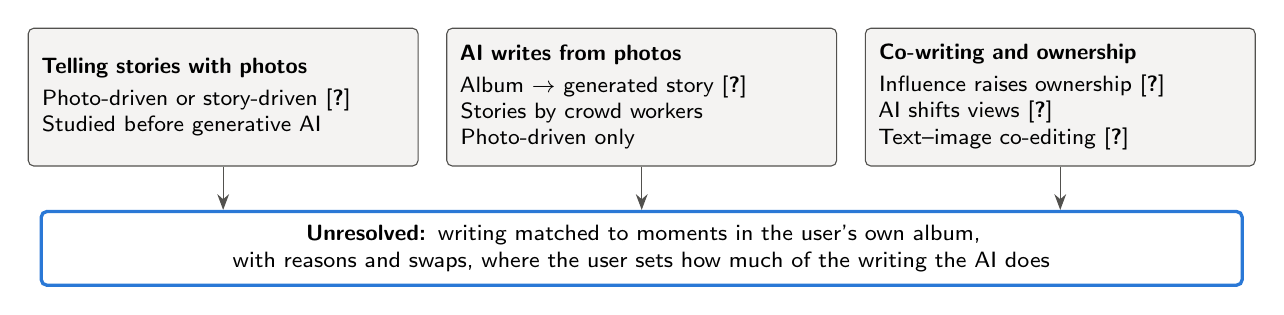
\begin{tikzpicture}[
  font=\sffamily\footnotesize,
  box/.style={draw=inkmuted, rounded corners=2pt, fill=gridline!45,
              text width=4.6cm, align=left, inner sep=5pt,
              minimum height=1.75cm, anchor=north},
  gap/.style={draw=accent, very thick, rounded corners=2pt, fill=white,
              text width=14.9cm, align=center, inner sep=5pt},
  arr/.style={-{Stealth[length=2mm]}, inkmuted}]
\node[box] (a) {\textbf{Telling stories with photos}\\[2pt]
  Photo-driven or story-driven \cite{balabanovic_storytelling_2000}\\
  Studied before generative AI};
\node[box, right=0.35cm of a.north east, anchor=north west] (b) {\textbf{AI writes from photos}\\[2pt]
  Album $\rightarrow$ generated story \cite{huang_visual_2016}\\
  Stories by crowd workers\\
  Photo-driven only};
\node[box, right=0.35cm of b.north east, anchor=north west] (c) {\textbf{Co-writing and ownership}\\[2pt]
  Influence raises ownership \cite{draxler_ai_2024}\\
  AI shifts views \cite{jakesch_co-writing_2023}\\
  Text--image co-editing \cite{fu_vistoria_2026-1}};
\node[gap, below=0.55cm of b] (g) {\textbf{Unresolved:} writing matched to moments in the user's own album,\\
  with reasons and swaps, where the user sets how much of the writing the AI does};
\draw[arr] (a.south) -- (a.south |- g.north);
\draw[arr] (b.south) -- (g.north);
\draw[arr] (c.south) -- (c.south |- g.north);
\end{tikzpicture}
\caption{Literature map: three strands of related work and the question none of them addresses.}
\label{fig:map}
\end{figure}
%TC:endignore

\section{Gap or opportunity}

The AI work on photos starts from the photos and generates words for them. Yet
Balabanović et al.\ found that people sometimes start from the story they want
to tell and then look for photos that fit
it~\cite{balabanovic_storytelling_2000}. In the work I reviewed, no system lets
a person set how much of a post's writing the AI does, from AI-written to
entirely their own, and then matches that writing to moments in their own album,
meaning groups of photos taken close together. The co-writing studies vary AI
involvement in text-only or fictional tasks; none covers the end of the range
where the AI chooses the photos and the person writes every word. It is unknown
whether people find such matches meaningful, how ownership changes across the
range when the photos are their own, whether a short reason per match makes
correction easier, as found for other tasks~\cite{kulesza_principles_2015}, and
whether people correct matches at all, given that AI suggestions changed what
participants wrote~\cite{jakesch_co-writing_2023}. It
is also unclear how well a model can match a line such as ``I didn't want the
day to end'', which describes a feeling rather than anything visible in a photo.

\section{Possible contribution}

I propose this question: when a system matches writing to moments in a
person's own trip album, with a one-line reason and a swap for each match, how
do match quality and ownership change as the writing moves from AI-written, to
AI suggestions the person accepts or rejects, to entirely their own? Outcomes
would be perceived match quality, sense of ownership (adapting the measures of
Draxler et al.~\cite{draxler_ai_2024}) and willingness to post.

The intended application is a tool for turning a trip album into social media
posts, where the person decides how much of the writing the AI does and can see
which words are the AI's, since people rarely declare AI authorship
themselves~\cite{draxler_ai_2024}.

Initial limits: the scope is trip albums and short writing; a first study would
be small and use participants' own photos, raising consent and privacy issues;
and weak matching on abstract lines may limit what it can show.

%TC:ignore
\bibliographystyle{abbrv}
\bibliography{references}
%TC:endignore

\end{document}
